\chapter{Related Work}
\label{chap:related_work}
This chapter provides an overview of the existing literature on art tracking with IoT and blockchains, highlighting previous research, methods, and findings related to the research question. Lastly, we discuss the reviewed literature and conclude the chapter by identifying research gaps.

\section{Artwork Conservation}
When it comes to preserving artworks, several factors play a role. This includes their exposition of human factors and environmental variations \cite{woodenartworkmonitoring}. More specifically, factors that can hamper artwork integrity include humidity, temperature, light, pollutants, and microbiological organisms \cite{riskassessment}. Usually, temperature and humidity are the most sensitive parameters \cite{riskassessment}. Monitoring such factors can be of significant importance when it comes to artwork preservation and health \cite{environmentmonitoring}. In addition to the conservation of artworks in museums or galleries, there is also the aspect of ensuring the safety of artwork during transportation. 

\section{Artwork Transportation}
Collections of artworks have been exhibited for generations. More often than not, artworks are showcased at different venues worldwide. The dangers imposed on artwork during transportation have been thoroughly researched and led to the development of innovative packaging and other safety measures \cite{artintransit}. Today, there exist a number of companies that specialize in the transportation of artwork \cite{kraftels, hasenkamp, weltifurrer}. The advertised solution often involves shock-absorbing as well as climate-controlled packaging. Even though these packaging solutions have been adequately tested, many reviewed companies rely on customer trust regarding their effectiveness in real-world applications. This presents an opportunity for monitoring systems leveraging the potential of emerging technologies to improve the artwork transportation process further.

\section{Artwork Monitoring Systems}
Technological advancements have made it possible to study the impacts of transportation on the integrity of artwork in more detail. Numerous studies have been conducted regarding this matter. One study utilized a small logging device to gather information on shock and vibrations generated during transportation \cite{shockvibrationtransit}. The study found that during the several dozen transportations monitored, the artwork suffered significant shock and vibration, even though the latest packaging techniques and appropriate means of transportation were used. This demonstrates that continuous monitoring of these parameters can be useful when verifying the integrity of the artwork after transportation.

In this context, \cite{woodenartworkmonitoring} proposes a real-time system that collects information about the artwork's environment and its safety conditions. This information can then be used to determine the quality of the conditions of artworks. The system uses a low-cost \gls{iot} node that can operate with very low power consumption, thus allowing for the realization of pervasive monitoring systems. This proposed system demonstrates how violations can be detected as they happen or have already happened. 

The study by \cite{pactart} goes one step further and proposes a proactive approach to potential violations. The so-called PACT-ART architecture employs advanced computing techniques like data mining and business process intelligence to predict the future state of the process. PACT-ART can then point out any possible violations and recommend actions to mitigate the misbehavior. \cite{riskmonitoring} expands on this and presents a system allowing for continuous risk assessment during storage, handling, transport, and exhibition.

\section{Artwork Management and Documentation}
Correct and secure information about artworks is one of the main concerns in the art world \cite{bcartmarket}. New technologies, such as blockchain, have been proposed as promising solutions to increase artworks' transparency, traceability, validity, and provenance \cite{cyberartmarket}. Especially smart contracts and \glspl{nft} have demonstrated the potential of blockchain technology to revolutionize the art world. 

\textcite{nftopportunities} has shown the benefits of \glspl{nft} protecting digital assets by proving their existence and ownership. \textcite{creativeindustry} has suggested the application of \glspl{nft} beyond digital art, proposing to physically tag an \gls{iot} device to an artwork or sculpture to transfer and track ownership. The \gls{iot} device is designed such that an attempt to tamper with the device will result in a blockchain record. This would potentially reduce intermediaries by providing a verifiable certificate that proves ownership, custodial history, and authenticity of a physical asset.

Platforms such as \textcite{artory}, \textcite{4art}, and \textcite{verisart} have already started to deploy blockchain and are offering a way to digitally register an artwork, introducing transparency and authenticity to the artwork, its history, and provenance \cite{bcartmarket}.


\textcite{artchain}, for example, developed a blockchain-based trading system for artworks that uses \glspl{nft} to represent physical artworks introducing traceability, irreversibility, and transparency into the art market. In this regard, \textcite{nftminter} has proposed an advanced \gls{nft} Minter for a blockchain-based artwork trading system. Besides trading, the work by \textcite{artrentalblockchain} developed an artwork rental system based on blockchain technology. The work is a proposal for a complete application of blockchain in the field of art leasing, which allows renters to securely and transparently browse and rent the available artworks.
 
\section{Applications of Blockchain and IoT}
\gls{scm} is another area where \gls{iot} is being used to improve processes. Similar to monitoring the environment around an artwork, \gls{iot} is being used in \gls{scm} to monitor the product state to ensure the right quality \cite{iotsupplychains}. Another technology that is innovating \gls{scm} is using blockchain. The combination of these two technologies in industrial systems and supply chains has been a "hot trend" in recent years \cite{industryiot}. Blockchain presents an opportunity to build trust with its unique immutability characteristic. This can be used to improve documentation and traceability of physical assets and ensure the authenticity of the asset and collected data. The work that follows has already been established in this context.

\textcite{modum.io} present a solution to monitor relevant environmental data while transporting medical products. Upon delivery, the collected data is checked for compliance by a smart contract and then stored on the blockchain. There, the data is immutable and verifiable by any party. The proposed system comprises backend, frontend, and \gls{iot} sensor devices. The architecture and components of the system are shown in Figure \ref{fig:modum.io}. In addition to the Ethereum blockchain network, modum.io uses a relational database to store raw temperature data and user credentials. The mobile clients download the temperature data via Bluetooth from the sensors and submit it to the server, which sends it to the \gls{sc} to evaluate the regulatory compliance and store the result on-chain.

\begin{figure}[ht]
    \centering
    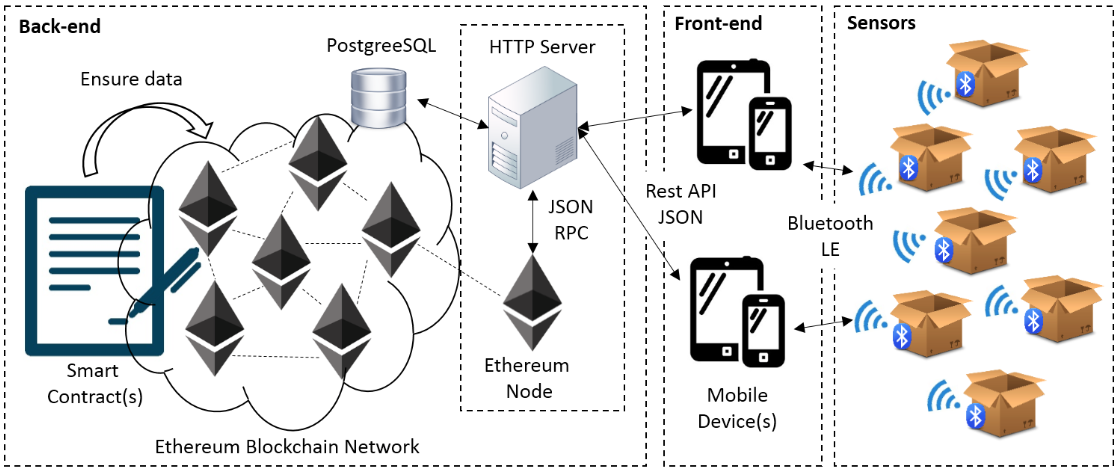
\includegraphics[width=0.8\textwidth]{diagrams/modum_architecutre.png}
    \caption{Modum.io AG Blockchain Architecture \cite{modum.io}}
    \label{fig:modum.io}
\end{figure}

\textcite{authena}, is a Swiss-based company that provides a platform for tracking and verifying the authenticity of physical assets using blockchain technology and \gls{iot}. Their platform offers three main products:
\begin{itemize}
    \item AUTHENA SHIELD: A tamper-proof end-to-end authenticity solution.
    \item AUTHENA L1VE: Real-time tracking of location and environmental conditions across countries and distribution channels.
    \item AUTHENA M3TA: Creating a secure link between physical product and its twin in the Metaverse.
\end{itemize}
According to \cite{authenahandelszeitung}, the system developed by authena can track the location as well as environmental data of an asset. This data is then stored securely and traceably on the blockchain. Unfortunately, the system is not open source, and the company provides no technical insight regarding the system's architecture.

\textcite{everledger}, is a digital transparency company providing technology solutions to increase transparency in global supply chains. They use blockchain to track and verify the authenticity of high-value assets such as diamonds, wine, and art. Their platform allows users to track the entire lifecycle of an asset, from production to ownership, using a secure and transparent blockchain-based ledger. Everledger mainly focuses on fraud detection, verification, and provenance records by issuing digital certificates stored on a private blockchain.

\section{Discussion}
\label{sec:related_work_discussion}
This literature review has shown that the art world's conservation of artwork remains a concern. This concern is increased when it comes to the transportation of artworks. The integrity and health of an artwork depend on a number of factors, including the environment surrounding the artwork. Besides shock and vibration, temperature and humidity are suggested to be the most sensitive parameters.

With new technologies like \gls{iot}, it becomes possible to monitor environmental parameters continuously. Multiple papers have already demonstrated the potential benefits of artwork monitoring \cite{pactart, riskmonitoring, woodenartworkmonitoring, shockvibrationtransit}. These benefits include the verification of packaging techniques and registration of any potential disturbances to the environment that could damage an artwork. We have also seen that the gathered data from artwork monitoring can be used to predict future violations and suggest actions to prevent damage.

On the other hand, we have reviewed the existing literature on blockchain opportunities in the art world. The main benefits include increased transparency and traceability by generating a secure chain of ownership and simplified verification of authenticity.

When combining the two technologies, we have seen substantial research in the area of \gls{scm}. Within \gls{scm}, subprocesses often involve the transportation of assets while ensuring their integrity and health. This can be very similar to the requirements of artwork transportation. However, little to no literature was found on the combination of \gls{iot} and blockchain in artwork logistics. The reviewed literature suggests that the benefits of both technologies can be combined to improve the current process of artwork transportation.
